\subsection{New public-data task domains}
\label{sec:new-public-tasks}
We add six tasks in three domains: raw-text classification (20 Newsgroups
and SMS Spam), structured-data classification (Adult and Spambase), and inverse
imaging (Optdigits denoising and missing-pixel completion)
\cite{sklearn20newsdata,uci2011sms,uci1996adult,uci1999spambase,uci1998optdigits}.
The two inverse tasks share the same image corpus and constitute two settings
within one domain, not two independent task-family replications. Dataset and
split definitions are fixed before formal training.

\begin{figure*}[htbp]\centering
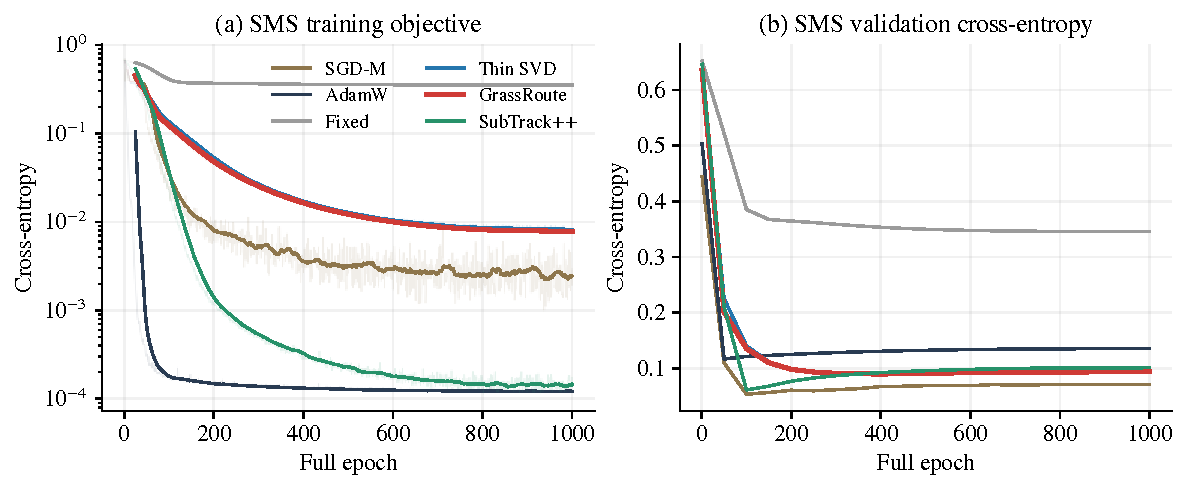
\includegraphics[width=\linewidth]{figures/fig_newtask_losses_selected.pdf}
\caption{SMS memory--quality operating point, with all six validation-selected methods. Left: the full 1000-epoch training objectives (raw losses faint, 25-epoch trailing means solid). Right: all saved validation cross-entropies. Hyperparameters were selected by final validation macro-F1; secondary cross-entropy did not replace that criterion. The full primary-metric matrix and every classifier endpoint remain in Tables~\ref{tab:newtasks-full} and~\ref{tab:newtasks-secondary}.}
\label{fig:newtasks-selected}
\end{figure*}


Every task compares SGD-M, AdamW, fixed routing, thin periodic SVD,
GrassRoute, and pinned official SubTrack++. All six receive nine 200-epoch
validation candidates and a fresh 1000-epoch selected run. Each epoch passes
through the complete training split in one full-data update. The routed grids
explicitly vary the residual/parallel learning-rate ratio across
$\{1,10,100\}$, since an SGD residual and an adaptive branch need not have
the same useful step-size scale. This changes the search protocol relative to
the original extension and is not silently pooled with it.

The periodic comparator directly factorizes the gradient matrix,
$G=L\Sigma V^\top$, and uses its top right singular vectors. This avoids
forming the full $G^\top G$ and transports both the first moment and the
diagonal second moment. Fixed and periodic methods store no unused routing
momentum. The complete search, sources and data hashes are frozen in the
new-task protocol; Appendix~\ref{app:new-task-full} reports every outcome.

The main-text subset uses an explicit reporting rule. A primary-metric gain
requires a better final held-out score than both AdamW and thin periodic SVD
after all six methods finish. A separate memory--quality trade-off requires
at least 50\% less state than AdamW, a primary classification score within
0.01 or an image MSE within 5\%, and a nondominated score--state point among
the six methods. The corresponding quality cost is stated explicitly. These are descriptive
one-seed criteria; statistical significance is not estimated.
The new public-data suite has completed 36 of 36 selected formal runs and 6 of six full comparisons. No completed new task currently establishes the predeclared gain over both AdamW and thin periodic SVD. Separate Pareto-efficient memory--quality trade-offs satisfy the predefined quality band on SMS / TF-IDF MLP. All attempted tasks and outcomes, including numerical failures and unfinished cells, remain in Appendix~\ref{app:new-task-full}; none is deleted after observing test results.

\par
% WWW table style: three rules, bold headers, reference green highlight.
\begin{table}[t]\centering\footnotesize
\caption{\textbf{SMS memory--quality trade-off.} Validation macro-F1 selects the configurations; test CE is secondary. The complete six-task comparison is in Table~\ref{tab:newtasks-full}. Persistent state is decimal MB.}
\label{tab:newtasks-selected}
\setlength{\tabcolsep}{5pt}
\reviewfit{\begin{tabular}{lrrr}\toprule {\bfseries Method} & {\bfseries F1 $\uparrow$} & {\bfseries Test CE $\downarrow$} & {\bfseries State MB $\downarrow$}\\\midrule
AdamW  &  95.48  &  0.1752  &  1.050\\
Thin SVD  &  94.29  &  0.0952  &  0.071\\
\rowcolor{oursbg}\textbf{GrassRoute} &  94.63  &  0.0931  &  0.137\\
\bottomrule\end{tabular}}\end{table}


On SMS, GrassRoute retains 0.137 MB versus AdamW's 1.050 MB (87.0\% less), with macro-F1 94.63 versus 95.48. Its separately retained test cross-entropy is 0.0931 versus 0.1752, and AUROC is 99.08 versus 98.28. These secondary probabilistic-quality observations did not determine the selected hyperparameters or redefine the primary F1 criterion. Every classifier endpoint is retained in Table~\ref{tab:newtasks-secondary}.

With the seed-42 validation choices frozen, the three new SMS initializations yield 94.74\% mean macro-F1 for GrassRoute, 95.48\% for AdamW and 94.29\% for thin periodic SVD. The GrassRoute state is 87.0\% smaller than AdamW's; its mean F1 is 0.74 points below AdamW. The one-point quality band holds in 1/3 seeds, and GrassRoute exceeds periodic SVD in 2/3 seeds. This is a descriptive mean memory--quality trade-off, with visible seed variability. All seeds and SGD appear in Table~\ref{tab:focused-sms-replication}.\par

\par
